\documentclass[12pt]{article}

\usepackage{amsmath}
\usepackage{amssymb}
\usepackage{calc}
\usepackage{units}
\usepackage{graphicx}
\usepackage[pdftex]{hyperref}
\usepackage{subfig}
\usepackage[margin=1in]{geometry}
\usepackage{listings}
\usepackage[numbers,sort&compress]{natbib}
\usepackage{bm}
\usepackage{paralist}
\usepackage[draft]{fixme}
\usepackage{textcomp}
\usepackage{yorkdefs}

\newcommand{\halflife}{\ensuremath{T_{\nicefrac{1}{2}}}\xspace}

\hypersetup{
  breaklinks=true,
  pdftitle={Alternating Current RLC Circuits},
  pdfauthor={Kevin R. Lynch based on a lab by D.C.Jain}, 
  pdfsubject={Phyiscs, Electricity and magnetism},
  pdfkeywords={resistance, inductance, capacitance, alternating current},
  pdflang={en-US},
}

\title{Alternating Current RLC Circuits}
\author{}
%Kevin R. Lynch, based on an earlier lab by D.C.Jain
%\date{2012-03-20}
\date{}

\begin{document}

\maketitle

\section{Objectives}
\label{sec:objectives}

\begin{enumerate}
\item To understand the voltage/current phase behavior of RLC circuits
  under applied alternating current voltages,
\item To understand the current amplitude behavior of RLC circuits
  under applied alternating current voltages, and
\item To understand the phenomenon of resonance in RLC circuits.
\end{enumerate}

\section{Introduction}
\label{sec:introduction}

\begin{figure}
  \centering
  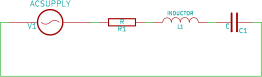
\includegraphics[width=2\textwidth/3]{figures/rlc-circuit}
  \caption{The RLC circuit.}
  \label{fig:rlccircuit}
\end{figure}
In previous labs\footnote{\textit{Alternating Current RC Circuits}
  and \textit{Alternating Current RL Circuits}} you studied the
behavior of the RC and RL circuits under alternating applied (or AC)
voltages.  Here, you will study the behavior of a similar circuit
containing series connected capacitor, inductor, and resistor; see
Figure~\ref{fig:rlccircuit}.

\section{Theory}
\label{sec:theory}

Once again, let's analyze this circuit using Kirchoff's Rules.  As
always, you find
\begin{gather*}
  V_s(t) - V_R(t) - V_L(t) - V_C(t) = 0\ ,
\end{gather*}
leading to a differential equation we have not encountered in these
labs before
\begin{gather*}
  \deriv[2]{q(t)}{t} + \frac{R}{L} \deriv{q(t)}{t} + \frac{1}{LC} q(t)
  = V_s(t)\ .
\end{gather*}
We will not actually solve this equation, as the derivation is beyond
the mathematics level of this course; however, in
Appendix~\ref{sec:solutions} we quote some important results.  For a
sinusoidally varying source voltage
\begin{gather*}
  V_s(t) = V_s \cos\omega t\ ,
\end{gather*}
we find the current is again out of phase, but this time, whether the
current lags or leads the applied voltage depends on whether the
inductive or capacitive reactances (both defined as before) dominate
the behavior of the circuit at the driving voltage.  Comparing the
solutions in the Appendix with our differential equation here,
matching coefficients, we have
\begin{align*}
  \omega_0 &= \frac{1}{\sqrt{LC}} & 2\beta &= \frac{R}{L}\ .
\end{align*}
Putting all these definitions together, we can solve for the current
and voltage profiles as a function of frequency
\begin{gather*}
  I(t) = \frac{V_s \omega}{L} 
  \frac{\cos\left(\omega t + \delta\right)}
  {\sqrt{\left(\omega_0^2-\omega^2\right)^2 +
      \left(2\beta\omega\right)^2}}\\ 
  V_R(t) = I(t) R = V_s 2\beta\omega 
  \frac{\cos\left(\omega t + \delta\right)}
  {\sqrt{\left(\omega_0^2-\omega^2\right)^2 +
      \left(2\beta\omega\right)^2}}\\
  V_C(t) = q(t)/C = 
  V_s \omega_0^2 \frac{\sin\left(\omega t + \delta\right)}
  {\sqrt{\left(\omega_0^2-\omega^2\right)^2 +
      \left(2\beta\omega\right)^2}}\\ 
  V_L(t) = -L\deriv[2]{q(t)}{t} = 
  V_s \omega^2 \frac{\sin\left(\omega t + \delta\right)}
  {\sqrt{\left(\omega_0^2-\omega^2\right)^2 +
      \left(2\beta\omega\right)^2}}\\ 
\end{gather*}
where the phase is given by 
\begin{gather*}
  \tan \delta = \frac{\omega_0^2-\omega^2}{2\beta\omega}\ .
\end{gather*}

The circuit impedance is given by
\begin{gather*}
  Z^2 = R^2 + \left(X_L-X_C\right)^2\ ,
\end{gather*}
which has all the same consequences for the voltage amplitudes as it
did for the $RC$ and $RL$ circuits.  We could rewrite these equations
in terms of these reactances (that's mostly left to you; see the
Pre-Lab exercises), but here we'll only discuss the phase.  You can
show
\begin{gather*}
  \tan \delta = \frac{X_L - X_C}{R}\ .
\end{gather*}

\fixme{Need to rethink these }
\begin{figure}
  \centering
  \subfloat[][Phases]{
%    \includegraphics[width=\textwidth/2-0.1in]{figures/frequency-phase}
  }
  \subfloat[][Voltage Amplitudes]{
%    \includegraphics[width=\textwidth/2-0.1in]{figures/frequency-amplitudes}
  }
  \caption{The phase angle as a function of angular frequency is on
    the left, while the voltage amplitudes are displayed on the right.
    In both cases, the frequency is normalized in units of $\omega_0 =
    1/\sqrt{LC}$.  The phase is normalized to $\pi/2$, while the
    amplitudes are normalized to $V_s$.}
  \label{fig:frequency}
\end{figure}
Just as we did for the RC and RL circuits, we should consider the
behavior of the RLC circuit as a function of frequency \ldots and
we're in for some new surprises. Consider first the phase.  Notice
that $\delta=0$ when $X_L = X_C$.  This is called the \textit{phase
  resonance} of the circuit.  At what frequency does this happen?
\begin{gather*}
  X_L = X_C = \omega_R L = \frac{1}{\omega_R C} \longrightarrow
  \omega_R = \frac{1}{\sqrt{LC}} = \omega_0\ .
\end{gather*}
This is called the \textit{natural} frequency of the circuit.  


There are a number of other resonances for this circuit.  We can, for
instance, also look for the maxima of the voltage amplitudes, the so
called \textit{amplitude resonances} of the circuit.  To predict
these, we extremize the amplitudes versus the frequencies
($\deriv{A(t)}{\omega} = 0$).  Clearly the current and the voltage
across the resistor will be maximized at the same frequency:
\begin{gather*}
  \left.\deriv{V_R(\omega)}{\omega}\right|_{\omega_R} = 0
  \longrightarrow \omega_R = \omega_0\ ,
\end{gather*}
or the \textit{current amplitude resonance} occurs at the same
frequency as the natural oscillation frequency of the circuit.
Interestingly, the amplitude resonance for the capacitor and inductor
voltages are \textit{not} the same as for the current!  For the
capacitor,
\begin{gather*}
  \left.\deriv{V_C(\omega)}{\omega}\right|_{\omega_C} = 0 
  \longrightarrow \omega_C = \sqrt{\omega_0^2 -
      \nicefrac{1}{2}(2\beta)^2}\ ,
\end{gather*}
the resonant voltage amplitude across the capacitor occurs at a
\textit{lower} frequency than the phase resonance!  For the inductor,
\begin{gather*}
  \left.\deriv{V_L(\omega)}{\omega}\right|_{\omega_L} = 0 
  \longrightarrow \omega_L = \sqrt{
      \frac{\omega_0^4}{\omega_0^2 - \nicefrac{1}{2}(2\beta)^2}
    }\ .
\end{gather*}
the resonant voltage amplitude occurs at a frequency \textit{higher}
than the phase resonance.  Of course, these last two resonance
conditions will only occur if the radical is real.

\section{Procedures}
\label{sec:procedures}

You should receive two multimeters (one of which should be a
BK-5460), an oscilloscope, a function generator, a
decade resistance box, a decade capacitance box, and an inductor.

\begin{enumerate}
\item First, select component values for testing.  Select a frequency
  between \unit[300]{Hz} and \unit[600]{Hz}, and a value for $C$
  between $\unit[0.06]{\mu F}$ and $\unit[0.1]{\mu F}$.  Calculate $X
  = \left| X_L-X_C \right|$ and choose a value for $R \approx 1.2 X$.
  Measure and record the values of $R$, the inductor resistance $R'$,
  and $C$.  Record the value of the inductance.
\item Configure the circuit for testing shown in
  Figure~\ref{fig:rlccircuit}.  Insert the Simpson multimeter to
  record the AC current.
\item Using the BK Precision meter, record the frequency $f$, and the
  RMS AC voltages across the signal generator $V_s$, the resistor
  $V_R$, the capacitor $V_C$, and the inductor $V_L$.  Are these
  values consistent?
\item \label{item:phase} Measure the phase shift between the current
  and applied voltage for your chosen frequency.  Connect the
  oscilloscope so as to measure the voltage across the resistor and
  signal generator; make sure the negtive inputs share a common
  reference point.  Make sure the two signal baselines are centered
  with respect to the horizontal and vertical axes of the
  oscilloscope, and adjust the voltage and time scales so that
  slightly more than one cycle of both waveforms is visible.  Measure
  the phase shift as you did in the previous lab.  Increase the
  frequency by 50\%, and determine the phase shift again.  Half the
  initial frequency, and repeat.
\item \label{item:phase_resonance} Next, find the resonant frequency.
  First, predict the value.  Then, go searching for it experimentally.
  There are three methods to do this:
  \begin{enumerate}
  \item Find the frequency which maximizes the current, 
  \item Find the frequency which eliminates the phase shift in AB
    mode, and
  \item Find the frequency which collapses the XY mode Lissajous
    figure to a line.
  \end{enumerate}
  In an ideal world each method should give the same result, although
  the last method is both easiest and most accurate.  Do they, in
  fact, produce the same result?
\item \label{item:amplitude_resonance} \fixme{Search for amplitude
    resonances of VC and VL}
\item \label{item:current_response} Next, map out the amplitude of the current
  response.  Without changing $R$ or $C$, vary the frequency over, say, ten
  points, and record the frequency, RMS voltage $V_s$ and RMS current
  $I$ at those points.  The low frequency should be half the
  resonance, the high frequency should be twice the resonance, and the
  middle point should be at the resonance.
\end{enumerate}

\appendix

\section{Derivation of Solutions}
\label{sec:solutions}

Applying Kirchoff's rules to the series RLC circuit leads to a second
order linear differential equation with constant coefficients, with a
driving function.  We won't solve this function in all its glory as we
did for the first order equation that arises for the RC and RL
equations.  In fact, solving the equation is somewhat beyond the level
of the prerequisite mathematics for this course, so we'll just quote
the solution here.\footnote{Although you can look up the solution
  methods on the net, or in any standard sophomore level physics or
  mathematics text.  I take the notation and solutions from Marion and
  Thornton's \textit{Classical Dynamics}.}

Let's write the differential equation in the form
\begin{gather*}
  \deriv[2]{q(t)}{t} + 2 \beta \deriv{q(t)}{t} + \omega_0^2 q(t) = A
  \cos\omega t\ .
\end{gather*}
A full solution to this equation can be written in terms of two
functions: 
 \begin{enumerate}
\item The ``complementary'' or ``homogeneous'' solution $q_c(t)$, when
  $A=0$.  This is the transient solution, and decays away
  exponentially; we'll not dwell on this any further.
\item The ``particular'' solution $q_p(t)$, where we don't drop the
  driving term.  We previously called this one the ``steady state''
  solution.  Typically, we take ``trial solutions'' of the same form
  as the driving term, and see if we can come work up a function that
  satisfies the equation.
\end{enumerate}
Let's try a particular solution that's a sinusoid.  Before diving in,
let's think about the \textit{form} of the physical solution that
we're looking for here.  In our specific problem, the solution to the
differential equation is the charge on the capacitor, but the physics
we're interested in is the phase difference between the
\textit{current} and the drive voltage.  Thus, we want a current that
is of the same functional form as the drive voltage.  Since we choose
a drive voltage that is a $\cos$, and current is the derivative of the
charge, we want to choose a steady state (particular) solution of the
form
\begin{gather*}
  q_p(t) = D \sin\left( \omega t + \delta \right)\ .
\end{gather*}
To show this is a solution, we need to find $D$ and $\delta$, which we
do by substituting into the differential equation, and we obtain
\begin{gather*}
  -D\omega^2 \sin\left(\omega t + \delta\right) + 2\beta D\omega
  \cos\left(\omega t + \delta\right) + D\omega_0^2 \sin\left(\omega t
    + \delta\right) = A \cos\omega t\ .
\end{gather*}
Next, we expand the $\sin$ and $\cos$ terms, since:
\begin{align*}
  \cos(a+b) &= \cos\omega t \cos\delta - \sin\omega t \sin\delta &
  \sin(a+b) &= \sin\omega t \cos\delta + \cos\omega t \sin\delta\ ,
\end{align*}
which gives six terms on the left, half of which contain a $\sin\omega
t$ and the other have contain $\cos\omega t$.  The right hand side
contains only $\cos\omega t$.  If this is a solution, the coefficients
of the $\sin\omega t$ and $\cos\omega t$ terms must separately be
equal, and must be collectively consistent.  Thus, we have two
equations for the two unknowns $D$ and $\delta$
\begin{gather*}
  \sin\omega t: \qquad -D\omega^2 \cos\delta - 2\beta D\omega
  \sin\delta + D\omega_0^2 \cos\delta = 0\\
  \cos\omega t: \qquad -D\omega^2 \sin\delta + 2\beta D\omega
  \cos\delta + D\omega_0^2 \sin\delta = A\ .
\end{gather*}
The $\sin\omega t$ equation can be solved for $\delta$
\begin{gather*}
  \tan\delta = \frac{\omega_0^2 - \omega^2}{2\beta\omega}\ .
\end{gather*}
Now that we have $\delta$, we can use the second equation to solve for
$D$
\begin{gather*}
  D = \frac{A}{\left(\omega_0^2-\omega^2\right) \sin\delta +
    2\beta\omega \cos\delta}\ .
\end{gather*}
How do we substitute for $\delta$ in this latter equation?  Using the
trigonometric relations
\begin{align*}
  \tan\delta &= \frac{\sin\delta}{\cos\delta} & 
  \sin^2\delta + \cos^2 \delta &= 1\ ,
\end{align*}
you can show that
\begin{align*}
  \sin\delta &= \frac{\omega_0^2 -
    \omega^2}{\sqrt{\left(\omega_0^2-\omega^2\right)^2 +
      \left(2\beta\omega\right)^2}} & 
  \cos\delta &=
  \frac{2\beta\omega}{\sqrt{\left(\omega_0^2-\omega^2\right)^2 + 
      \left(2\beta\omega\right)^2}}\ .
\end{align*}
Substituting these values, you will obtain the coefficient $D$
\begin{gather*}
  D = \frac{A}{\sqrt{\left(\omega_0^2-\omega^2\right)^2 + 
      \left(2\beta\omega\right)^2}}\ .
\end{gather*}


\newpage
 
\section*{Pre-Lab Exercises}

Answer these questions as instructed on Blackboard; make sure to
submit them before your lab session!

\fixme{Need new pre-lab exercises}
\begin{enumerate}
\item Calculate the reactance of a $\unit[7]{H}$ capacitor at a
  frequency of \unit[250]{Hz}.
% 11 kOhm
\item If an RL circuit has a $\unit[50]{\Omega}$ resistor in series
  with a $\unit[7]{m H}$ inductor, what will its impedance be at
  \unit[500]{Hz}?
% 54.6 Ohm
\item An RL circuit has a $\unit[5]{k\Omega}$ resistor and a
  $\unit[1]{H}$ inductor.  At what frequency will the current
  lag the voltage by $\pi/4$?
% 800 Hz
\item An RL circuit has a $\unit[5]{k\Omega}$ resistor and a
  $\unit[1]{m H}$ inductor.  This circuit is driven by a
  \unit[100]{Hz} sine wave with \unit[1]{V} amplitude.  What is the
  amplitude of the current in the circuit?
% 0.20 mA
\end{enumerate}

\newpage

\section*{Post-Lab Exercises}

\fixme{need new post-lab exercises}
\begin{enumerate}
\item From your recorded inductance, and the measured resistance,
  capacitance, and initial frequency, determine the reactance and
  impedance of your circuit.  Make sure to estimate your
  uncertainties.  Determine the impedance experimentally via another
  method, taking care of the uncertaintites.% V_s/I
  Do you get the same results?
\item Estimate the uncertainties on the measured values of $V_s$,
  $V_L$, $V_C$, and $V_R$.  Are these values consistent with each
  other?  Explain what you mean by ``consistent''.
\item From your measurements in Step~\ref{item:phase} of the
  procedure, determine the phase shift at each of the three measured
  frequencies, including an estimate of the uncertainty.  How do these
  compare to the theoretical predictions? 
\item Are your three measurements of the phase resonance frequency
  consistent with each other?  With the prediction?  
\item Describe qualitatively what happens to your signals when you
  vary the frequency around the phase resonance.
\item \fixme{Amplitude resonances?}
\item Is your data from Step~\ref{item:current_response} consistent with the
  predictions of theory?  Specifically, do the voltage and current
  amplitudes measured by oscilloscope and by multimeter match, within
  uncertainties, and do they comport with theoretical expectations?
\item Discuss briefly whether you have met the objectives of the lab
  exercises.
\end{enumerate}

\end{document}

%%% Local Variables: 
%%% mode: latex
%%% TeX-master: t
%%% End: 
